% !TeX spellcheck = en_US


\chapter{Infrastructure}


\section{Overview}
The system infrastructure takes care of real-time collection, processing, and visualization of sensor data.
The architecture comprises three main entities: the whisker platform, the controller, and the actuator.
The platform provides two I2C buses for reading sensor data, each equipped with three MLX90393 sensors.
The sensors are connected in a daisy chain via a QUIK connector.
This allows to avoid the need for soldering.
Theoretically, up to 16 sensors can be connected per bus, but we are using only three, as the development boards are limited to four sensors per bus.
As the controller device a Raspberry Pi 5 is chosen, as it has sufficient processing power and is small enough to be mounted on the robotic arm.
Currently, the actuator is simulated; however, it will eventually be replaced by a robotic arm.
Figure~\ref{fig:infrastructure_overview} summarizes the system architecture.

\begin{figure}[htb]
    \centering
    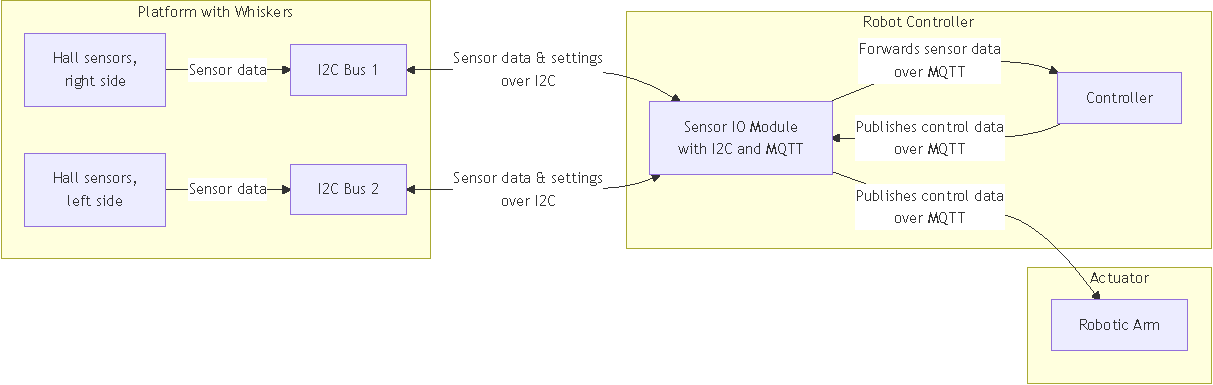
\includegraphics[width=\textwidth]{figures/diagrams/infrastructure-overview}
    \caption{Overview of the system infrastructure.}
    \label{fig:infrastructure_overview}
\end{figure}


\section{Controller}
The control loop of the system is depicted in Figure~\ref{fig:control-flow}.
This loop continuously processes sensor data, evaluates control policies, and generates control messages.
Figure~\ref{fig:control-hierarchy} illustrates the hierarchy of components within the controller.

\begin{figure}
    \centering
    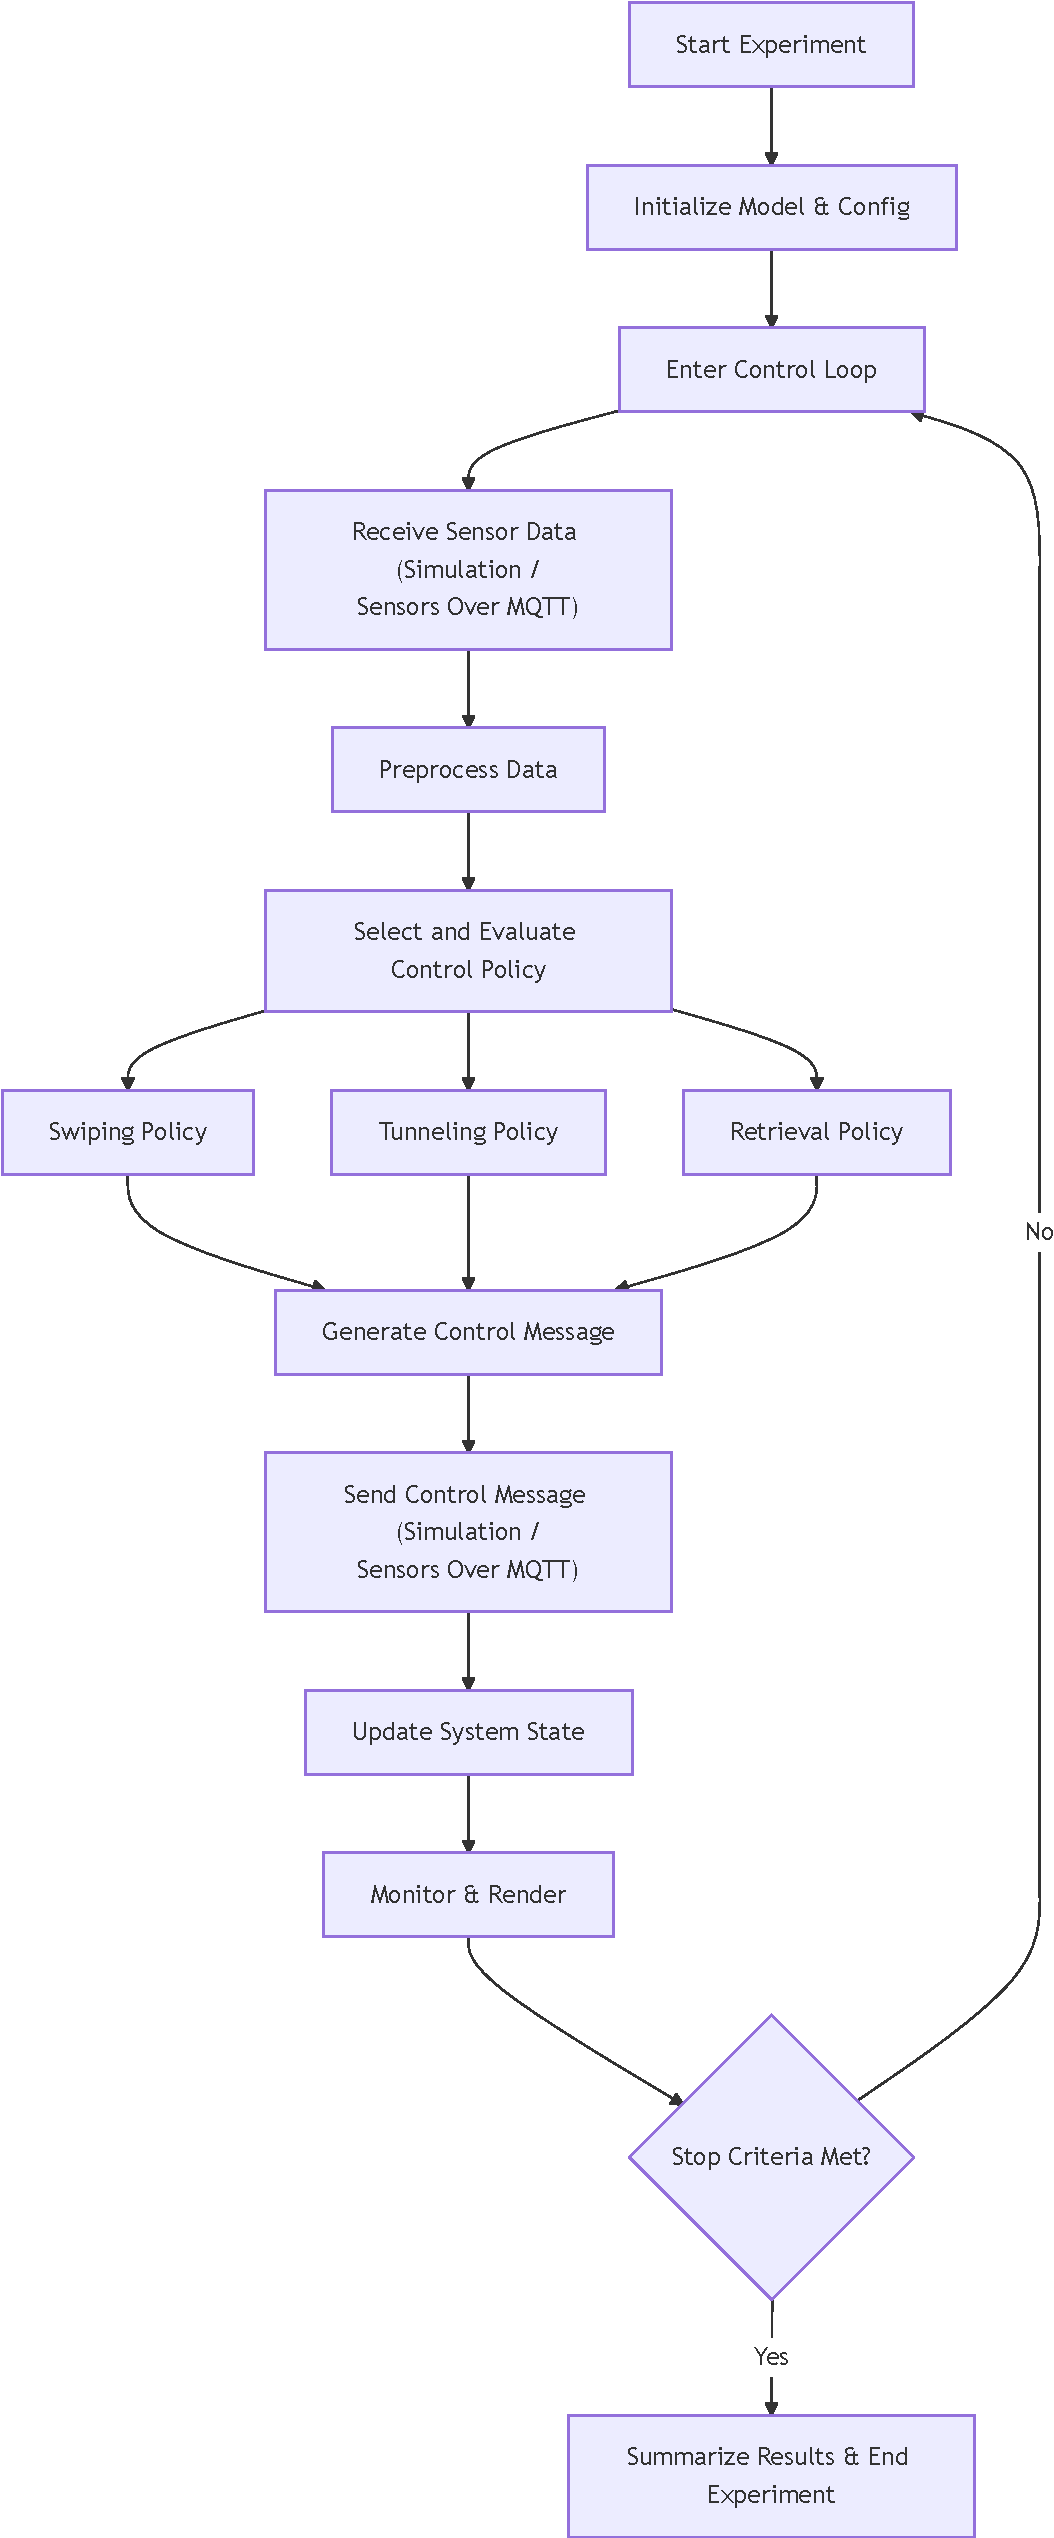
\includegraphics[height=\textheight]{figures/diagrams/control-flow}
    \caption{Data flow in the system infrastructure.}
    \label{fig:control-flow}
\end{figure}


\section{Simulation}
The simulation framework is used for testing the controller.
It provides a realistic physics engine environment for validating control algorithms.
The simulation is based on MuJoCo, a physics engine developed by Google DeepMind.
Figure~\cref{fig:mujoco} shows the simulation interface of MuJoCo.

\begin{figure}
    \centering
    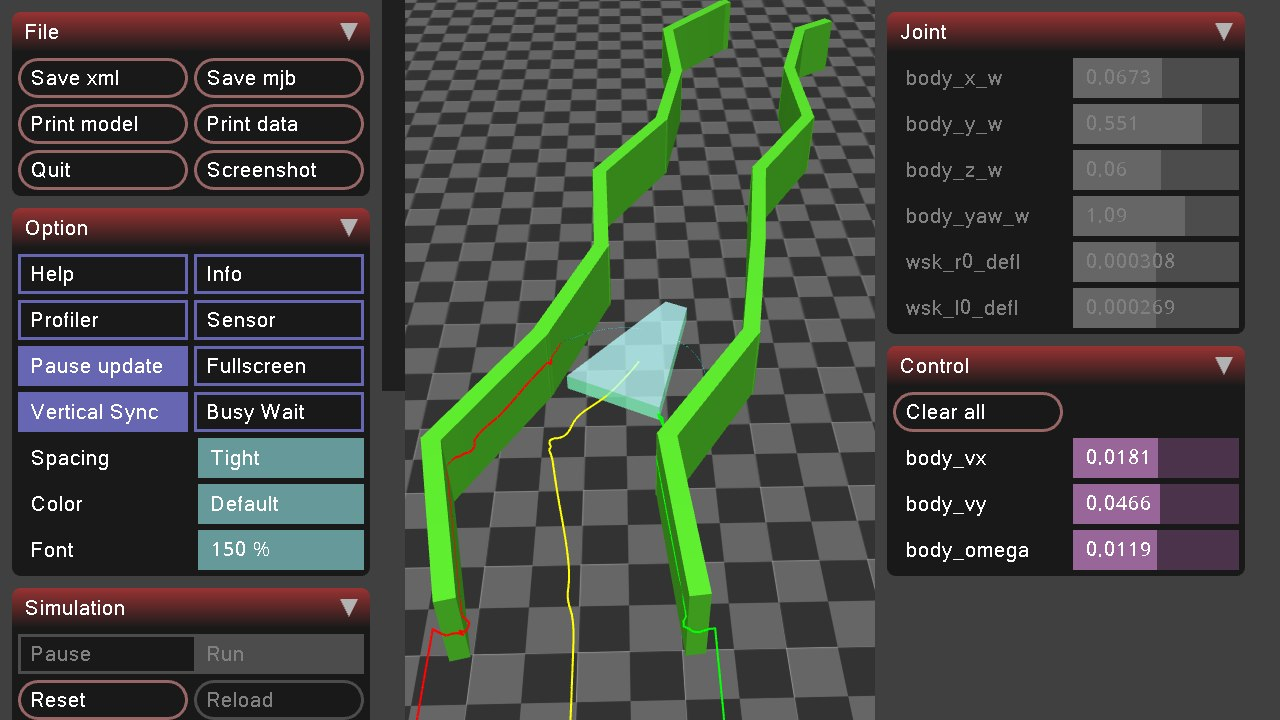
\includegraphics[width=\textwidth]{figures/mujoco}
    \caption{Simulation interface of the MuJoCo physics engine.}
    \label{fig:mujoco}
\end{figure}

The simulation framework is designed to be modular, and so the controller has no dependency on the simulation framework.
That makes possible the integration of new frameworks or sensor data sources and sinks.
10 test cases are provided to test the performance of 3 different policies.
For each test case the results are automatically evaluated and plotted, similar to figures~\ref{fig:experiment-disk-swiping}--\ref{fig:experiment-round-tunnel-swiping-tunneling}.
For each test case an accompanying video is provided, which shows the simulation in action.
MuJoCo allows to follow, pause and analyze the simulation.
The simulation is set up in a way that the trajectories of the whisker tips and the platform center of mass are displayed continuously.
This is a sort of sanity check for the simulation, as the deflection model and tip calculations are error-prone.


\section{System Services}
The system is composed of several interconnected services, as illustrated in Figure~\ref{fig:data_flow}.
All of them are running in Docker containers, as to guarantee a consistent and separate environment across different machines.
They are orchestrated using Docker Compose, which simplifies the setup and configuration.
The control system runs on any machine with Docker installed, like Raspberry Pi 5, making it easy to deploy.

\begin{figure}
    \centering
    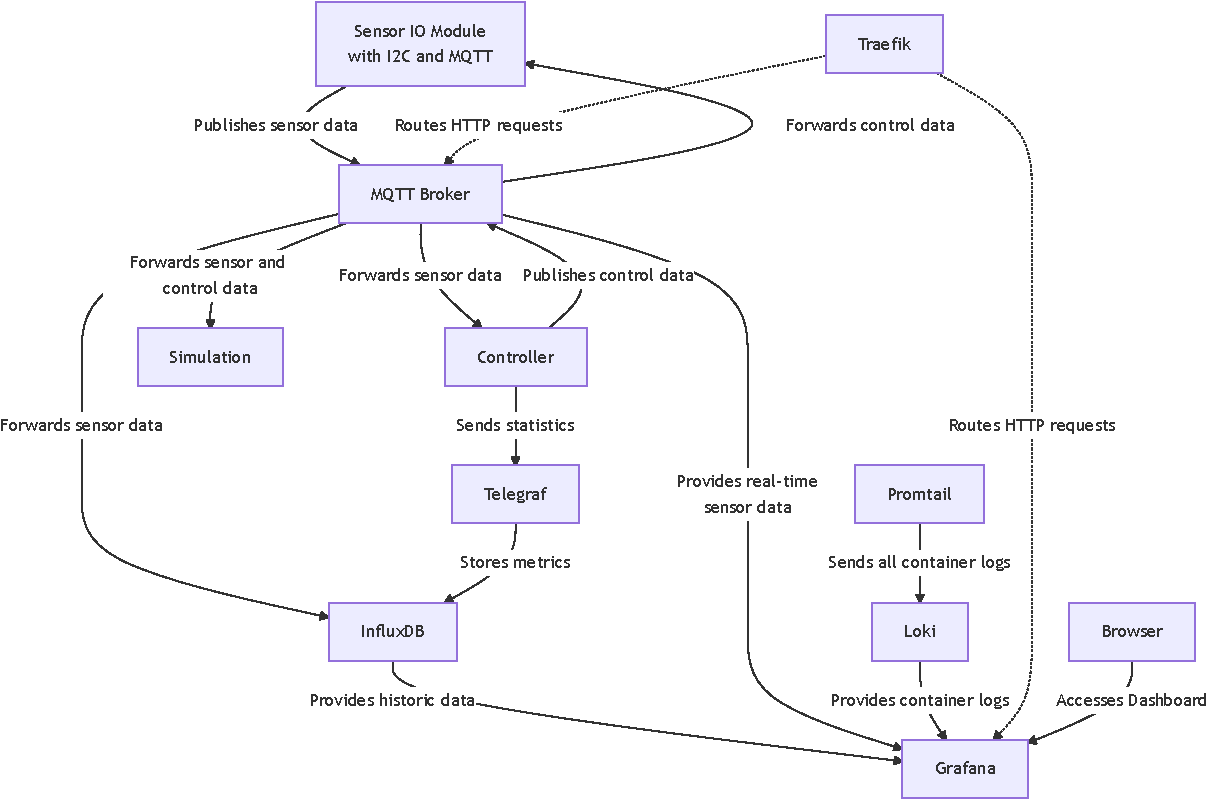
\includegraphics[width=\textwidth]{figures/diagrams/infrastructure-robot-controller}
    \caption{Data flow in the system infrastructure.}
    \label{fig:data_flow}
\end{figure}

\begin{itemize}
    \item \textbf{Sensor IO Module:}
    This module reads sensor data from the robot's I2C buses and publishes the data via MQTT.
    It also forwards control commands from the controller to the actuator.
    Currently, the built-in I2C buses of the Raspberry Pi are used for simplicity.
    But generally speaking, the Sensor IO module can be decoupled from the controller and run on a separate device.

    \item \textbf{Controller:}
    The Controller processes sensor data and generates control signals.
    It also publishes statistics for further monito ring.

    \item \textbf{MQTT Broker:}
    Acting as the central messaging hub, the MQTT Broker receives and distributes sensor and control data.
    It is based on the subscriber-publisher model.
    This component is critical for system responsiveness.

    \item \textbf{Telegraf:}
    Telegraf collects sensor data and controller performance metrics.
    The data is then forwarded to InfluxDB for storage.

    \item \textbf{InfluxDB:}
    InfluxDB is a time-series database, which is used to store historical sensor data and controller performance metrics.
    It serves as a persistent storage solution for the system during the execution of the experiments.

    \item \textbf{Grafana:}
    Grafana provides a web-based dashboard that visualizes the sensor data in real-time.
    It allows users to monitor the system's status interactively.

    \item \textbf{Promtail:}
    Promtail is responsible for collecting logs from the various services and forwarding them to Loki.

    \item \textbf{Loki:}
    Loki aggregates the logs provided by Promtail and makes them available for visualization via Grafana.
    This centralized logging system helps in troubleshooting and monitoring system health.

    \item \textbf{Traefik:}
    Traefik is used as a reverse proxy for communication between the services and with the outside world.
    For instance, it allows access to the Grafana dashboard via a web browser.
\end{itemize}


\section{Dashboard}
The system dashboard is built using Grafana, a powerful analytics and monitoring platform.
It provides a web-based interface for visualizing sensor data and control signals.
Grafana Live with MQTT is employed to transmit real-time system status.
Figure~\ref{fig:grafana} shows a minimalistic dashboard with magnetic data from six whisker sensors sampled in real-time.


\begin{figure}[htb]
    \centering
    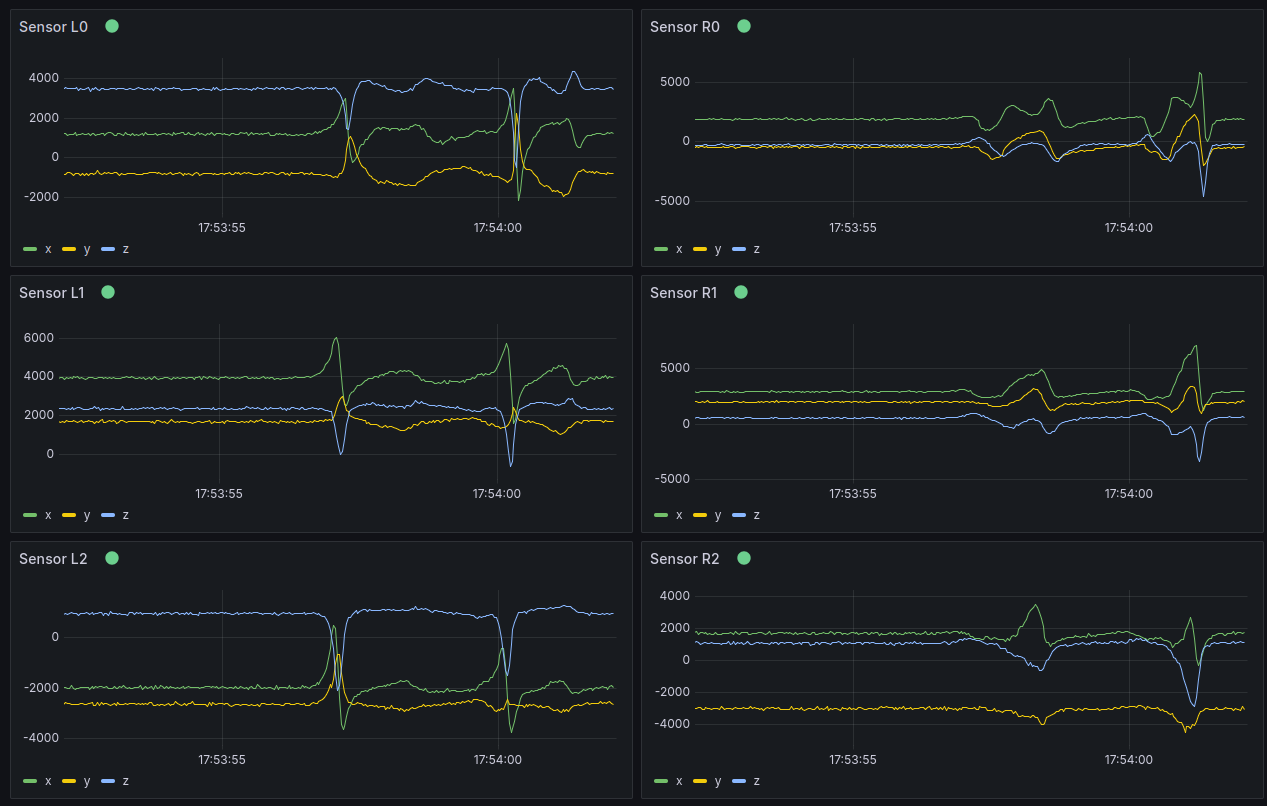
\includegraphics[width=\textwidth]{figures/grafana}
    \caption{Visualization of magnetic data of 6 whisker sensors in real time using Grafana.}
    \label{fig:grafana}
\end{figure}

The plans for the dashboard include:
\begin{itemize}
    \item Visualization of whisker deflection in 2D
    \item State machine visualization
    \item Performance metrics of the contour reconstruction algorithm
    \item System cycle time and overload monitoring
    \item Historical data analysis and trend monitoring.
\end{itemize}
